\documentclass[12pt]{article}

\usepackage{amsmath}
\usepackage{array}
\usepackage{caption}
\usepackage[top=1in, bottom=1in, left=0.75in, right=0.75in]{geometry}
\usepackage{graphicx}
\usepackage[colorlinks=true, allcolors=blue]{hyperref}
\usepackage[utf8]{inputenc}
\usepackage{multirow}
\usepackage[section]{placeins}

\graphicspath{{./figures/}}

\title{ECE 271: Chapter 2 Reading Report}
\author{Phi Luu}
\date{\today}

\begin{document}

\maketitle

%%%%%%%%%%%%%%%%%%%%%%%%%%%%%%%%%%%%%%%%%%%%%%%%%%%%%%%%%%%%%%%%%%%%%%%%%%%%%%%%
% Chapter Outline
%%%%%%%%%%%%%%%%%%%%%%%%%%%%%%%%%%%%%%%%%%%%%%%%%%%%%%%%%%%%%%%%%%%%%%%%%%%%%%%%
\section{Chapter Outline}

This chapter covers the basics of combinational logic design and heavily focuses on the functional and timing relationships between inputs and outputs of a circuit. In this chapter, the authors use boolean and boolean algebra to explain multilevel combinational logic and apply these concepts to make hardware reduction for more complex circuits. Another focus of this chapter is showing how to use Karnaugh maps (or K-maps) to minimize logic in a more graphical and intuitive way. Each of the mentioned topics will be discussed further throughout the following subsections.

%%%%%%%%%%%%%%%%%%%%%%%%%%%%%%%%%%%%%%%%
% Introduction
%%%%%%%%%%%%%%%%%%%%%%%%%%%%%%%%%%%%%%%%
\subsection{Introduction}

A \textit{circuit} is a network that processes discrete-valued variables. A circuit needs to have the following:

\begin{itemize}
    \item one or more discrete-valued \textit{input} terminals
    \item one or more discrete-valued \textit{output} terminals
    \item a \textit{functional specification} describing the relationship between the inputs and the outputs
    \item a \textit{timing specification} describing the delay between the changes in the inputs and the responses of the outputs
\end{itemize}

A circuit can be viewed as a black box similar to Figure~\ref{figure:1} below:

\begin{figure}[h]
    \centering
    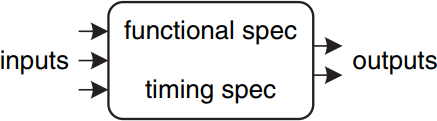
\includegraphics[width=0.3\textwidth]{circuit.png}
    \caption{A circuit as a black box with inputs, outputs, and specifications}
    \label{figure:1}
\end{figure}

\newpage

A circuit has two components:

\begin{itemize}
    \item \textit{Elements}: An element is itself a circuit with inputs, outputs, and specifications.
    \item \textit{Nodes}: A node is a wire whose voltage is discrete-valued. Nodes are further classified into three types:
    \begin{itemize}
        \item \textit{Inputs} receive values from the external world.
        \item \textit{Outputs} deliver values to the external world.
        \item \textit{Internals} are wires that are neither inputs nor outputs.
    \end{itemize}
\end{itemize}

Digital circuits are classified as \textit{combinational} or \textit{sequential}. A combinational circuit is memoryless; its outputs depend only on the current values of the inputs. Recall the logic gates from chapter 1, they are examples of a combinational circuit. A sequential circuit, on the other hand, has memory; its outputs depend on both the current values of the inputs and the previous values of the inputs. This chapter focuses on combinational circuits, and chapter 3 will cover sequential circuits.

A circuit is combinational if it consists of interconnected circuit elements such that

\begin{itemize}
    \item Every circuit element is combinational.
    \item Every node is either an input to the circuit or connected to \textit{exactly one} output terminal of an element.
    \item There are no cyclic paths.
\end{itemize}

The functional specification of a circuit is often expressed as a truth table or a Boolean equation which will be discussed in the next subsection.

%%%%%%%%%%%%%%%%%%%%%%%%%%%%%%%%%%%%%%%%
% Boolean Equations
%%%%%%%%%%%%%%%%%%%%%%%%%%%%%%%%%%%%%%%%
\subsection{Boolean Equations}

\begin{enumerate}
    %%%%%%%%%%%%%%%%%%%%
    % Terminology
    %%%%%%%%%%%%%%%%%%%%
    \item \textbf{Terminology}

    Boolean equations deal with variables that are either TRUE or FALSE. Therefore, they are perfect for describing digital logic. Table~\ref{table:1} below shows the terminologies, notations, and truth tables of some commonly used Boolean equations.

    \begin{table}[h]
        \centering
        \begin{tabular}{ | c | >{\centering\arraybackslash}p{6em} | >{\centering\arraybackslash}p{2em} | >{\centering\arraybackslash}p{2em} | >{\centering\arraybackslash}p{4em} | }
        \hline \rule{0em}{1em}
        \textbf{Terminology}                              & \textbf{Notation}          & \multicolumn{3}{c|}{\textbf{Truth Table}}                               \\ \hline \rule{0em}{1em}
        \multirow{3}{*}{Complement of $A$}                & \multirow{3}{*}{$\bar{A}$} & \multicolumn{2}{c|}{$\mathbf{A}$} & $\mathbf{\bar{A}}$                  \\ \cline{3-5} \rule{0em}{1em}
                                                        &                            & \multicolumn{2}{c|}{0}            & 1                                   \\ \cline{3-5} \rule{0em}{1em}
                                                        &                            & \multicolumn{2}{c|}{1}            & 0                                   \\ \hline \rule{0em}{1em}
        \multirow{5}{*}{Product/Implicant of $A$ and $B$} & $AB$                       & $\mathbf{A}$    & $\mathbf{B}$    & $\mathbf{AB}$                       \\ \cline{2-5} \rule{0em}{1em}
                                                        & $A$ AND $B$                & 0               & 0               & 0                                   \\ \cline{2-5} \rule{0em}{1em}
                                                        & \multirow{3}{*}{}          & 0               & 1               & 0                                   \\ \cline{3-5} \rule{0em}{1em}
                                                        &                            & 1               & 0               & 0                                   \\ \cline{3-5} \rule{0em}{1em}
                                                        &                            & 1               & 1               & 1                                   \\ \hline \rule{0em}{1em}
        \multirow{5}{*}{Sum of $A$ and $B$}               & $A + B$                    & $\mathbf{A}$    & $\mathbf{B}$    & $\mathbf{A + B}$                    \\ \cline{2-5} \rule{0em}{1em}
                                                        & $A$ OR $B$                 & 0               & 0               & 0                                   \\ \cline{2-5} \rule{0em}{1em}
                                                        & \multirow{3}{*}{}          & 0               & 1               & 1                                   \\ \cline{3-5} \rule{0em}{1em}
                                                        &                            & 1               & 0               & 1                                   \\ \cline{3-5} \rule{0em}{1em}
                                                        &                            & 1               & 1               & 1                                   \\
        \hline
        \end{tabular}
        \caption{Terminologies, notations, and truth tables of some Boolean equations}
        \label{table:1}
    \end{table}

    A \textit{minterm} is a \textbf{product} involving all variables of the inputs to the function. A \textit{maxterm} is a \textbf{sum} involving all variables of the inputs to the function.

    When multiple Boolean variables take part in a Boolean equation, the \textit{order of operations} is vital to determinant the result of the equation---similarly to the order of operations in decimal-based algebra. In Boolean equations, \textbf{NOT has the highest precedence, followed by AND, and then OR}. For instance, the Boolean equation:

    \begin{equation} \label{equation:1}
        Y = \bar{A}B + BC\bar{D}
    \end{equation}

    can be interpreted as
    \begin{equation} \label{equation:2}
        Y = ((\bar{A})B) + (BC(\bar{D})) = ((\text{NOT }A)\text{ AND }B)\text{ OR }(B\text{ AND }C\text{ AND }(\text{NOT }D))
    \end{equation}

    %%%%%%%%%%%%%%%%%%%%
    % Sum-of-Products Form
    %%%%%%%%%%%%%%%%%%%%
    \item \textbf{Sum-of-Products Form}

    A truth table of $N$ inputs contains $2^N$ rows. Each row is associated with a \textbf{minterm}---a product involving all inputs of the function---\textbf{that is TRUE for that row}. Take an unknown Boolean equation $Y$ as an example:

    \begin{table}[h]
        \centering
        \begin{tabular}{ | c | c | c | c | c | }
        \hline \rule{0em}{1em}
        $\mathbf{A}$ & $\mathbf{B}$ & $\mathbf{Y}$ & \textbf{Minterm} & \textbf{Minterm Name} \\ \hline \rule{0em}{1em}
        0            & 0            & 0            & $\bar{A}\bar{B}$ & $m_0$                 \\ \hline \rule{0em}{1em}
        0            & 1            & 1            & $\bar{A}B$       & $m_1$                 \\ \hline \rule{0em}{1em}
        1            & 0            & 0            & $A\bar{B}$       & $m_2$                 \\ \hline \rule{0em}{1em}
        1            & 1            & 1            & $AB$             & $m_3$                 \\ \hline
        \end{tabular}
        \caption{Minterms of an unknown Boolean equation $Y$}
        \label{table:2}
    \end{table}

    The minterm for the first row is $\bar{A}\bar{B}$ because $\bar{A}\bar{B}$ is TRUE when $A = 0$ and $B = 0$. Similarly, the minterm for the second row is $\bar{A}B$ because $\bar{A}B$ is TRUE when $A = 0$ and $B = 1$, and so on. Like arrays in most non-math programming languages (C, C++, Java, Javascript, Python, etc.), minterms are numbered starting with zero.

    A Boolean equation can be written for any truth table by summing each of the minterms for which the output, $Y$, is TRUE. This is called the \textbf{sum-of-products canonical form} of a function, denoted by a \textit{sigma notation}, $\Sigma$.

    From the truth table presented by Table~\ref{table:2}, the Boolean equation $Y$ can be solved using the sum-of-products canonical form, as follows:

    \begin{equation} \label{equation:3}
        Y = F(A, B) = \Sigma(m_1, m_3) = \Sigma(1, 3) = \bar{A}B + AB
    \end{equation}

    %%%%%%%%%%%%%%%%%%%%
    % Product-of-Sums Form
    %%%%%%%%%%%%%%%%%%%%
    \item \textbf{Product-of-Sums Form}

    This method is quite similar to the sum-of-products method. Each row is associated with a \textbf{maxterm}---a sum involving all inputs of the function---\textbf{that is FALSE for that row}. Reuse Table~\ref{table:2} and construct the maxterm columns:

    \begin{table}[h]
        \centering
        \begin{tabular}{ | c | c | c | c | c | }
        \hline \rule{0em}{1em}
        $\mathbf{A}$ & $\mathbf{B}$ & $\mathbf{Y}$ & \textbf{Maxterm}    & \textbf{Maxterm Name} \\ \hline \rule{0em}{1em}
        0            & 0            & 0            & $A + B$             & $M_0$                 \\ \hline \rule{0em}{1em}
        0            & 1            & 1            & $A + \bar{B}$       & $M_1$                 \\ \hline \rule{0em}{1em}
        1            & 0            & 0            & $\bar{A} + B$       & $M_2$                 \\ \hline \rule{0em}{1em}
        1            & 1            & 1            & $\bar{A} + \bar{B}$ & $M_3$                 \\ \hline
        \end{tabular}
        \caption{Maxterms of an unknown Boolean equation $Y$}
        \label{table:3}
    \end{table}

    The maxterm for the first row is $A + B$ because $A + B$ is FALSE when $A = 0$ and $B = 0$. Similarly, the minterm for the second row is $A + \bar{B}$ because $A + \bar{B}$ is FALSE when $A = 0$ and $B = 1$, and so on. Like minterms, maxterms are numbered starting with zero.

    A Boolean equation can be written for any truth table as the AND of maxterms for which the output, $Y$, is FALSE. This is called the \textbf{product-of-sums canonical form} of a function, denoted by a \textit{pi notation}, $\Pi$.

    From the truth table presented by Table~\ref{table:3}, the Boolean equation $Y$ can be solved using the product-of-sums canonical form, as follows:

    \begin{equation} \label{equation:4}
        Y = E(A, B) = \Pi(M_0, M_2) = \Pi(0, 2) = (A + B)(\bar{A} + B)
    \end{equation}

    It is recommended to use sum-of-products when the output has more TRUEs than FALSEs and use the product-of-sums when the output has more FALSEs than TRUEs.
\end{enumerate}

%%%%%%%%%%%%%%%%%%%%%%%%%%%%%%%%%%%%%%%%
% Boolean Algebra
%%%%%%%%%%%%%%%%%%%%%%%%%%%%%%%%%%%%%%%%
\subsection{Boolean Algebra}

\begin{enumerate}
    %%%%%%%%%%%%%%%%%%%%
    % Axioms
    %%%%%%%%%%%%%%%%%%%%
    \item \textbf{Axioms}

    \textit{Axioms} are statements or propositions assummed to be correct. They are unprovable in the sense that a definition cannot be proved.

    Table~\ref{table:4} below shows the axioms of Boolean algebra.

    \begin{table}[h]
        \centering
        \begin{tabular}{ | c | c | c | c | c | }
        \hline \rule{0em}{1em}
           & \textbf{Axiom}              &     & \textbf{Dual}              & \textbf{Name} \\ \hline \rule{0em}{1em}
        A1 & $B = 0\text{ if }B \neq 1$  & A1' & $B = 1\text{ if }B \neq 0$ & Binary field  \\ \hline \rule{0em}{1em}
        A2 & $\bar{0} = 1$               & A2' & $\bar{1} = 0$              & NOT           \\ \hline \rule{0em}{1em}
        A3 & $0 \cdot 0 = 0$             & A3' & $1 + 1 = 1$                & AND/OR        \\ \hline \rule{0em}{1em}
        A4 & $1 \cdot 1 = 1$             & A4' & $0 + 0 = 0$                & AND/OR        \\ \hline \rule{0em}{1em}
        A5 & $0 \cdot 1 = 1 \cdot 0 = 0$ & A5' & $1 + 0 = 0 + 1 = 1$        & AND/OR        \\ \hline
        \end{tabular}
        \caption{Axioms of Boolean algebra}
        \label{table:4}
    \end{table}

    Based on these axioms, all the theorems of Boolean algebra can be proven.

    %%%%%%%%%%%%%%%%%%%%
    % Theorems of One Variable
    %%%%%%%%%%%%%%%%%%%%
    \item \textbf{Theorems of One Variable}

    Table~\ref{table:5} below shows the theorems of one variable in Boolean algebra.

    \begin{table}[h]
        \centering
        \begin{tabular}{ | c | c | c | c | c | }
        \hline \rule{0em}{1em}
           & \textbf{Theorem}      &     & \textbf{Dual}       & \textbf{Name} \\ \hline \rule{0em}{1.25em}
        T1 & $B \cdot 1 = B$       & T1' & $B + 0 = B$         & Identity      \\ \hline \rule{0em}{1.25em}
        T2 & $B \cdot 0 = 0$       & T2' & $B + 1 = 1$         & Null Element  \\ \hline \rule{0em}{1.25em}
        T3 & $B \cdot B = B$       & T3' & $B + B = B$         & Idempotency   \\ \hline \rule{0em}{1.25em}
        T4 & \multicolumn{3}{c|}{$\bar{\bar{B}} = B$}          & Involution    \\ \hline \rule{0em}{1.25em}
        T5 & $B \cdot \bar{B} = 0$ & T5' & $B + \bar{B} = 1$   & Complements   \\ \hline
        \end{tabular}
        \caption{Boolean theorems of one variable}
        \label{table:5}
    \end{table}

    %%%%%%%%%%%%%%%%%%%%
    % Theorems of Several Variables
    %%%%%%%%%%%%%%%%%%%%
    \item \textbf{Theorems of Several Variables}

    Table~\ref{table:6} below shows the theorems of several variables in Boolean algebra

    \begin{table}[]
        \centering
        \begin{tabular}{| c | c | c | c | c |}
        \hline \rule{0em}{1.25em}
            & \textbf{Theorem}                                                                                                            &      & \textbf{Dual}                                                                                                                & \textbf{Name}                                                 \\ \hline \rule{0em}{1.25em}
        T6  & $B \cdot C = C \cdot B$                                                                                                     & T6'  & $B + C = C + B$                                                                                                              & Commutativity                                                 \\ \hline \rule{0em}{1.25em}
        T7  & $(B \cdot C) \cdot D = B \cdot (C \cdot D)$                                                                                 & T7'  & $(B + C) + D = B + (C + D)$                                                                                                  & Associativity                                                 \\ \hline \rule{0em}{1.25em}
        T8  & $(B \cdot C) + (B \cdot D) = B \cdot (C + D)$                                                                               & T8'  & $(B + C) \cdot (B + D) = B + (C \cdot D)$                                                                                    & Distributivity                                                \\ \hline \rule{0em}{1.25em}
        T9  & $B \cdot (B + C) = B$                                                                                                       & T9'  & $B + (B \cdot C) = B$                                                                                                        & Covering                                                      \\ \hline \rule{0em}{1.25em}
        T10 & $(B \cdot C) + (B \cdot \bar{C}) = B$                                                                                       & T10' & $(B + C) \cdot (B + \bar{C}) = B$                                                                                            & Combining                                                     \\ \hline \rule{0em}{1.25em}
        T11 & \begin{tabular}[c]{@{}c@{}}$(B \cdot C) + (\bar{B} \cdot D) + (C \cdot D)$\\ $= B \cdot C + \bar{B} \cdot D$\end{tabular}   & T11' & \begin{tabular}[c]{@{}c@{}}$(B + C) \cdot (\bar{B} + D) \cdot (C + D)$\\ $= (B +C) \cdot (\bar{B} \cdot D)$\end{tabular}     & Consensus                                                     \\ \hline \rule{0em}{1.25em}
        T12 & \begin{tabular}[c]{@{}c@{}}$\overline{B_0 \cdot B_1 \cdot B_2 ...}$\\ $= \bar{B_0} + \bar{B_1} + \bar{B_2}...$\end{tabular} & T12' & \begin{tabular}[c]{@{}c@{}}$\overline{B_0 + B_1 + B_2 ...}$\\ $= \bar{B_0} \cdot \bar{B_1} \cdot \bar{B_2} ...$\end{tabular} & \begin{tabular}[c]{@{}c@{}}De Morgan's\\ Theorem\end{tabular} \\ \hline
        \end{tabular}
        \caption{Boolean theorems of several variables}
        \label{table:6}
    \end{table}

    According to De Morgan's theorem, a NAND gate is equivalent to an OR gate with inverted inputs, and a NOR gate is equivalent to an AND gate with inverted inputs.

    %%%%%%%%%%%%%%%%%%%%
    % The Truth Behind It All
    %%%%%%%%%%%%%%%%%%%%
    \item \textbf{The Truth Behind It All}

    Theorems can be proven based on axioms by several methods, two of which are using truth tables and using \textit{perfect induction}.

    %%%%%%%%%%%%%%%%%%%%
    % Simplifying Equations
    %%%%%%%%%%%%%%%%%%%%
    \item \textbf{Simplifying Equations}

    Using the theorems from Table~\ref{table:5} and Table~\ref{table:6}, Equation~\ref{equation:3} can be rewritten as

    \begin{equation} \label{equation:5}
        Y = \bar{A}B + AB = B\bar{A} + BA = B(\bar{A} + A) = B \cdot 1 = B
    \end{equation}

    and Equation~\ref{equation:4} can be rewritten as

    \begin{equation} \label{equation:6}
        Y = (A + B)(\bar{A} + B) = (B + A)(B + \bar{A}) = B + (A\bar{A}) = B + 0 = B
    \end{equation}

    Since Equation~\ref{equation:5} and Equation~\ref{equation:6} are equivalent, Equation~\ref{equation:3} and Equation~\ref{equation:4} are also equivalent. Thus, the sum-of-products and the product-of-sums methods yield the same results. Additionally, the truth table presented by Table~\ref{table:2} can be simplified to the Boolean equation $Y = \bar{B}$.

    An equation in the sum-of-products form is \textit{minimized} if it uses the fewest possible number of implicants, the minimal one is the one with the fewest literals. An implicant is called a \textit{prime implicant} if it cannot be combined with any other implicants in the equation to form a new implicant with fewer literals. Therefore, the implicants in a minimal equation must all be prime implicants.
\end{enumerate}

%%%%%%%%%%%%%%%%%%%%%%%%%%%%%%%%%%%%%%%%
% From Logic to Gates
%%%%%%%%%%%%%%%%%%%%%%%%%%%%%%%%%%%%%%%%
\subsection{From Logic to Gates}

A \textit{schematic} is a diagram of a digital circuit showing the elements and the wires that connect them together. For example, the schematic in Figure~\ref{figure:2} shows a possible hardware implementation of the logic function $Y = \bar{A}\bar{B}\bar{C} + A\bar{B}\bar{C} + A\bar{B}C$.

\begin{figure}[h]
    \centering
    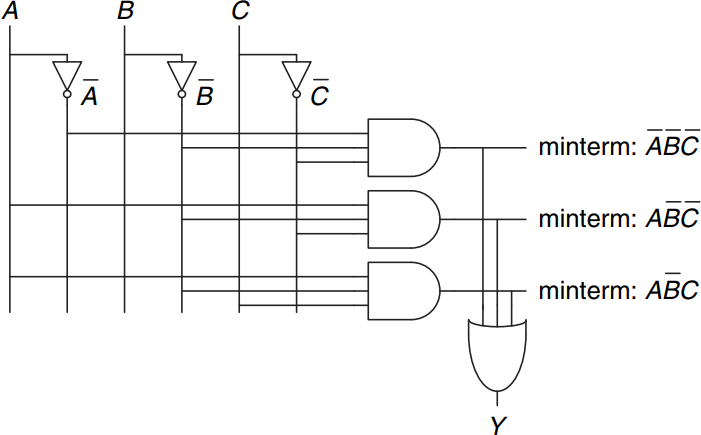
\includegraphics[width=0.5\textwidth]{schematic.png}
    \caption{A schematic of $Y = \bar{A}\bar{B}\bar{C} + A\bar{B}\bar{C} + A\bar{B}C$}
    \label{figure:2}
\end{figure}

There are several conventions to follow when drawing a schematic. Below is a list of a few of the guidelines:

\begin{itemize}
    \item Inputs are on the left (or top) side.
    \item Outputs are on the right (or bottom) side.
    \item Gates should follow from left to right if possible.
    \item Straight wires are usually better than wires with multiple corners.
    \item Wires always connect at a T junction.
    \item A dot where wires cross indicates a connection between the wires.
    \item Wires crossing \textit{without} a dot make no connection.
\end{itemize}

It is strongly recommended to reduce the logic function before implementing a schematic version of it.

%%%%%%%%%%%%%%%%%%%%%%%%%%%%%%%%%%%%%%%%
% Multilevel Combinational Logic
%%%%%%%%%%%%%%%%%%%%%%%%%%%%%%%%%%%%%%%%
\subsection{Multilevel Combinational Logic}

\begin{enumerate}
    %%%%%%%%%%%%%%%%%%%%
    % Hardware Reduction
    %%%%%%%%%%%%%%%%%%%%
    \item \textbf{Hardware Reduction}

    In reality, designers often build circuits with more than two levels of logic gates. These multilevel combinational circuits may use less hardware than their two-level counterparts. For example, an eight-input XOR would require 128 eight-input AND gates and one 128-input OR gate for a two-level sum-of-products implementation. A much better solution is to use a tree of seven two-input XOR gates, which drastically reduces the amount of hardware needed.

    %%%%%%%%%%%%%%%%%%%%
    % Bubble Pushing
    %%%%%%%%%%%%%%%%%%%%
    \item \textbf{Bubble Pushing}

    Bubble pushing is an intuitive way to redraw a circuit so that the bubbles cancel out and the function can be more easily determined. The guidelines for bubble pushing are as follows:

    \begin{itemize}
        \item Begin at the output and work toward the inputs.
        \item Push any bubbles on the final output back toward the inputs so that the equation can be expressed in terms of the output.
        \item Work backward: if the current gate has (or does not have) an input bubble, draw the preceeding gate with (or without) an output bubble.
        \item According to De Morgan's theorem, NAND will be converted to OR with inverted inputs and NOR will be converted to AND with inverted inputs.
    \end{itemize}
\end{enumerate}

%%%%%%%%%%%%%%%%%%%%%%%%%%%%%%%%%%%%%%%%
% X's and Z's, Oh My
%%%%%%%%%%%%%%%%%%%%%%%%%%%%%%%%%%%%%%%%
\subsection{X's and Z's, Oh My}

Boolean algebra is limited to 0's and 1's. However, real circuits can also have illegal and floating values, denoted respectively by X and Z.

\begin{enumerate}
    %%%%%%%%%%%%%%%%%%%%
    % Illegal Value: X
    %%%%%%%%%%%%%%%%%%%%
    \item \textbf{Illegal Value: X}

    The symbol X indicates the circuit node has an \textit{unknown} or \textit{illegal} value. This commonly happens if it is being driven into both 0 and 1 at the same time---called \textit{contention}---like in Figure~\ref{figure:3} below:

    \begin{figure}[h!]
        \centering
        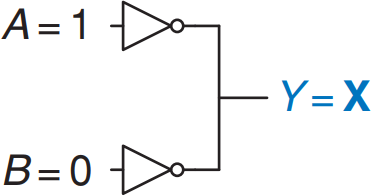
\includegraphics[width=0.15\textwidth]{circuit_with_contention.png}
        \caption{A circuit with contetion. Must avoid contention as it will damage the system.}
        \label{figure:3}
    \end{figure}

    %%%%%%%%%%%%%%%%%%%%
    % Floating Value: Z
    %%%%%%%%%%%%%%%%%%%%
    \item \textbf{Floating Value: Z}

    The symbol Z indicates a node is being driven \textit{neither} HIGH \textit{nor} LOW. The node is said to be \textit{floating}, \textit{high impedance}, or \textit{high Z}.

    A typical misconception is that a floating or undriven node is the same as a logic 0. In reality, it might be 0, might be 1, or might be ``floating" at some voltage in between. Figure~\ref{figure:4} below shows a tristate buffer and its truth table. The output of this buffer can be a HIGH, a LOW, or a Z.

    \begin{figure}[h!]
        \centering
        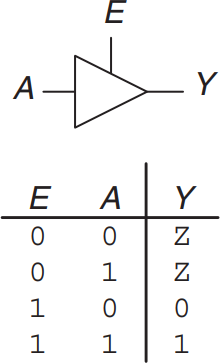
\includegraphics[width=0.15\textwidth]{circuit_with_floating.png}
        \caption{A circuit with a floating node.}
        \label{figure:4}
    \end{figure}
\end{enumerate}

%%%%%%%%%%%%%%%%%%%%%%%%%%%%%%%%%%%%%%%%
% Karnaugh Maps
%%%%%%%%%%%%%%%%%%%%%%%%%%%%%%%%%%%%%%%%
\subsection{Karnaugh Maps}

\textit{Karnaugh maps} (\textit{K-maps}) are a graphical method for simplifying Boolean equations, invented in 1953 by Maurice Karnaugh at Bell Labs. Karnaugh maps work well for problems with up to four variables. One of the strengths of Karnaugh maps is that they use the intuition to make Boolean equations' simplification more accurate.

\begin{enumerate}
    %%%%%%%%%%%%%%%%%%%%
    % Circular Thinking
    %%%%%%%%%%%%%%%%%%%%
    \item \textbf{Circular Thinking}

    Each of the rows of the truth table is represented by a single square of the K-map. The K-map also ``wraps around," which means the squares on the far right are adjacent to the squares on the far left and they differ only in one variable. Reading the minterms from the K-map is exactly equivalent to reading equations in sum-of-products form directly from the truth table, as shown in Figure~\ref{figure:5} below:

    \begin{figure}
        \centering
        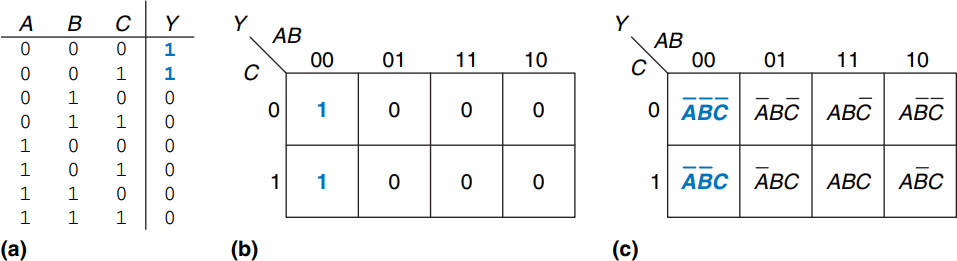
\includegraphics[width=0.65\textwidth]{truth_table_karnaugh_map.png}
        \caption{(a) truth table, (b) K-map, (c) K-map showing minterms of a three-input function.}
        \label{figure:5}
    \end{figure}

    \textbf{K-map reading direction: start from the top-left, then read top to bottom and then move to the column on the right.}

    Using the truth table, the sum-of-products form, and Boolean algebra, the given logic function can be expressed as

    \begin{equation} \label{equation:7}
        Y = \bar{A}\bar{B}\bar{C} + \bar{A}\bar{B}C = \bar{A}\bar{B}(\bar{C} + C) = \bar{A}\bar{B}
    \end{equation}

    Using the K-map, graphically \textbf{circle the minterms in adjacent square}:

    \begin{figure}
        \centering
        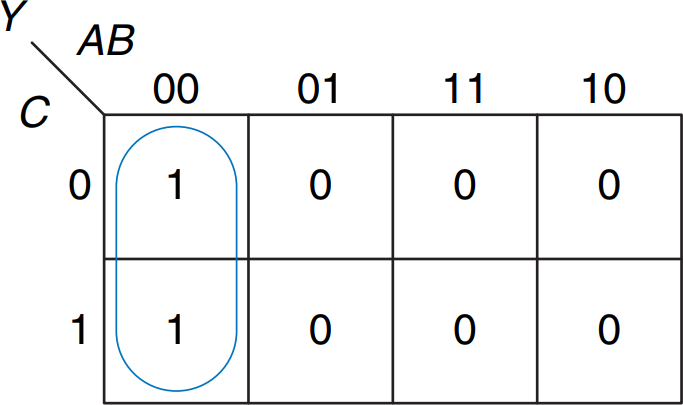
\includegraphics[width=0.3\textwidth]{kmap_minimization.png}
        \caption{K-map minimization.}
        \label{figure:6}
    \end{figure}

    For each circle, write a corresponding implicant (AND). Variables whose true \textit{and} complementary forms both appear in the circle are excluded from the implicant. In Figure~\ref{figure:6}, the variable $C$ is excluded from the implicant, leaving $Y = \bar{A}\bar{B}$---the same result as Equation~\ref{equation:7}.

    %%%%%%%%%%%%%%%%%%%%
    % Logic Minimization with K-Maps
    %%%%%%%%%%%%%%%%%%%%
    \item \textbf{Logic Minimization with K-Maps}

    K-maps provide an easy visual way to minimize logic. Follows the guidelines below to find a minimized equation from a K-map:

    \begin{itemize}
        \item Use the fewest circles possible to cover all the 1's.
        \item Everything in the circles must contain 1's.
        \item Each circle must span $2^n$ rectangular blocks.
        \item Each circle should be as large as possible.
        \item A circle may wrap around the edge of the K-map.
        \item A 1 in a K-map must be circled \textit{multiple times}, allowing fewer circles to be used.
    \end{itemize}

    %%%%%%%%%%%%%%%%%%%%
    % Don't Cares
    %%%%%%%%%%%%%%%%%%%%
    \item \textbf{Don't Cares}

    The ``don't care" entries in a truth table indicate some variables do not affect the output, denoted X. The ``don't care" entries can either be 0 or 1.

    X appear in truth table outputs where the value is unimportant or the corresponding input combination can never happen. These outpus can be treated by either 0's or 1's depending on the designer. In a K-map, X allows even more logic minimization.

    %%%%%%%%%%%%%%%%%%%%
    % The Big Picture
    %%%%%%%%%%%%%%%%%%%%
    \item \textbf{The Big Picture}

    Boolean algebra and Karnaugh maps are two methods of logic simplification. In modern engineering practice, \textit{logic synthesizers} are computer programs that produce simplified circuits from a description of a logic function much more efficiently than humans.
\end{enumerate}

%%%%%%%%%%%%%%%%%%%%%%%%%%%%%%%%%%%%%%%%
% Combinational Building Blocks
%%%%%%%%%%%%%%%%%%%%%%%%%%%%%%%%%%%%%%%%
\subsection{Combinational Building Blocks}

\begin{enumerate}
    %%%%%%%%%%%%%%%%%%%%
    % Multiplexer
    %%%%%%%%%%%%%%%%%%%%
    \item \textbf{Multiplexer}

    \textit{Multiplexers} are among the most commonly used combinational circuits. They choose an output from among several possible inputs based on the value of a \textit{select} signal. A multiplexer is often called a \textit{mux}.

    A multiplexer can be built from sum-of-products logic or from tristate buffers.

    Multiplexers can be used as \textit{lookup tables} to perform logic functions.

    %%%%%%%%%%%%%%%%%%%%
    % Decoders
    %%%%%%%%%%%%%%%%%%%%
    \item \textbf{Decoders}

    A decoder has $N$ inputs and $2^N$ outputs. It asserts \textit{exactly one} of its output depending on the input combination. The outputs are called \textit{one-hot}, as exactly one output is ``hot" (HIGH) at a given time.

    \begin{figure}[h]
        \centering
        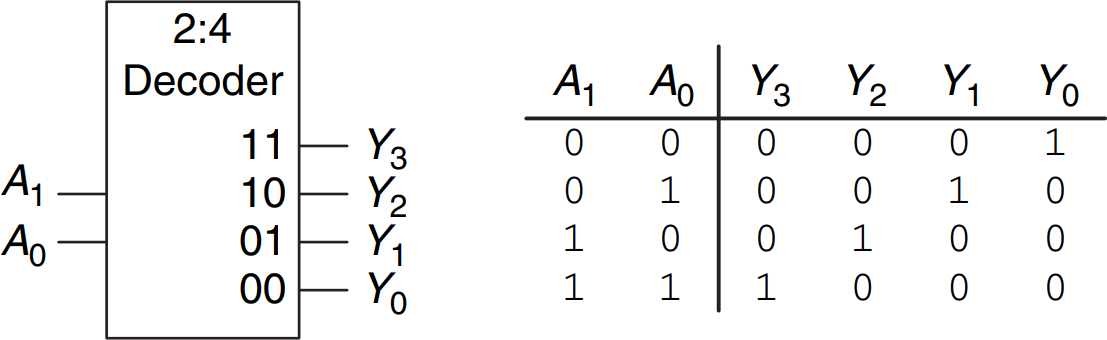
\includegraphics[width=0.5\textwidth]{decoder.png}
        \caption{A 2:4 decoder and its truth table.}
        \label{figure:7}
    \end{figure}
\end{enumerate}

%%%%%%%%%%%%%%%%%%%%%%%%%%%%%%%%%%%%%%%%
% Timing
%%%%%%%%%%%%%%%%%%%%%%%%%%%%%%%%%%%%%%%%
\subsection{Timing}

Previous subsections discuss the functional aspect of a circuit---that is, whether the circuit works ideally with the fewest gates. On the other hand, one of the most challenging issues in circuit design is \textit{timing}: making a circuit run \textit{fast}. This subsection focuses on this aspect of a circuit.

\begin{enumerate}
    %%%%%%%%%%%%%%%%%%%%
    % Propagation and Contamination Delay
    %%%%%%%%%%%%%%%%%%%%
    \item \textbf{Propagation and Contamination Delay}

    Combinational logic is characterized by its \textit{propagation delay} and \textit{contamination delay}. The \textbf{propagation delay} $t_{pd}$ is the \textbf{maximum} time from when an input changes until the output(s) reach their final value. The \textbf{contamination delay} $t_{cd}$ is the \textbf{minimum} time from when an input changes until any outputs starts to change its value.

    \begin{figure}[h]
        \centering
        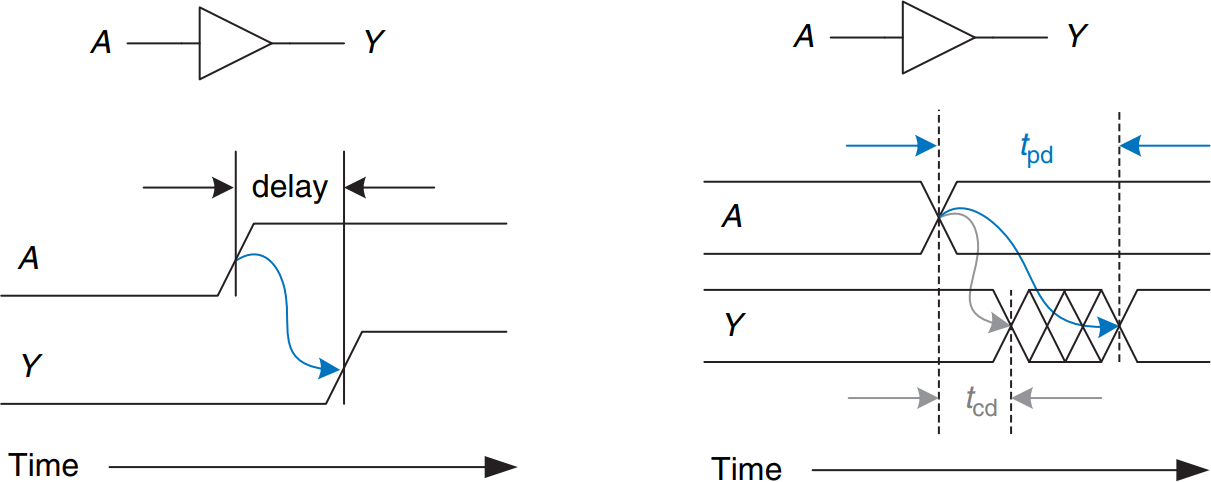
\includegraphics[width=0.5\textwidth]{propagation_contamination_delay.png}
        \caption{Propagation delay and contamination delay}
        \label{figure:8}
    \end{figure}

    %%%%%%%%%%%%%%%%%%%%
    % Glitches
    %%%%%%%%%%%%%%%%%%%%
    \item \textbf{Glitches}

    It is possible that a single input transistion can cause multiple output transistions. These are called \textit{glitches} or \textit{hazards}. Although glitches don't usually cause problems, it is important to realize they exist and recognize them when looking at the timing diagram.

    In general, a glitch can occur when a change in a single variable crosses the boundary between two prime implicants in a K-map. A glitch can be eliminated by covering these boundaries with redundant implicants---with the cost of extra hardware. However, simultaneous transitions on multiple inputs can also cause glitches---and these glitches cannot be fixed by adding hardware.
\end{enumerate}

%%%%%%%%%%%%%%%%%%%%%%%%%%%%%%%%%%%%%%%%
% Summary
%%%%%%%%%%%%%%%%%%%%%%%%%%%%%%%%%%%%%%%%
\subsection{Summary}

A digital circuit is a module with discrete-valued inputs and outputs and the functional and timing relationships between the two. This chapter has focused on combinational circuits---circuits that depend only on the current value of their inputs.

The function of a combinational circuit can be given by a truth table or a Boolean equation. A logic function can be written from the truth table using the sum-of-products or the product-of-sums methods.

Boolean equations can be simplified using Boolean algebra or Karnaugh maps. Logic simplification makes the logic function require less hardware, thus effectively reduce the cost of hardware implementation.

Logic gates are connected to form combinational circuits that perform the desired function. Any function in sum-of-products form can be built using two-level logic: NOT gates from the complements of the inputs, AND gates from the products, and OR gates from the sum. When using NAND and NOR, use bubble pushing to keep track of the inversions.

Logic gates are combined to produce larger circuits, such as multiplexers (mux), decoders, and priority circuits. A multiplexer can choose the data from a select input. A decoder sets one of the outputs HIGH depending on the inputs. A priority circuit produces an output indicating the highest priority input.

Timing is one of the most challenging issues in circuit design. The timing specification consists of the propagation and the contamination delay---indicating the longest and shortest time it takes for the outputs to change after the inputs change, respectively. There are many different ways to implement combinational circuits, and these ways offer trade-offs between speed and cost.

%%%%%%%%%%%%%%%%%%%%%%%%%%%%%%%%%%%%%%%%%%%%%%%%%%%%%%%%%%%%%%%%%%%%%%%%%%%%%%%%
% Grey Box Exploration
%%%%%%%%%%%%%%%%%%%%%%%%%%%%%%%%%%%%%%%%%%%%%%%%%%%%%%%%%%%%%%%%%%%%%%%%%%%%%%%%
\section{Grey Box Exploration}

\begin{enumerate}
    %%%%%%%%%%%%%%%%%%%%%%%%%%%%%%%%%%%%%%%%
    % First grey box
    %%%%%%%%%%%%%%%%%%%%%%%%%%%%%%%%%%%%%%%%
    \item The first blurb is on page 61, which states: \textit{The null element theorem leads to some outlandish statements that are actually true! It is particularly dangerous when left in the hands of advertisers: YOU WILL GET A MILLION DOLLARS or we'll send you a toothbrush in the mail. (You'll most likely be receiving a toothbrush in the mail.)}

    Usually, when people talks about advertisement, they often assess the truth of the advertised statements. The example provided by the blurb, ``YOU WILL GET A MILLION DOLLARS or we'll send you a toothbrush in the mail," is an advertised statement. To assess the true-false of this statement, Boolean algebra is required.

    Let the clause ``YOU WILL GET A MILLION DOLLARS" be a Boolean variable, called $A$. Let the clause ``we'll send you a toothbrush in the mail" be another Boolean variable, called $B$. Below is the truth table of $A\text{ OR }B$.

    \begin{table}[h]
        \centering
        \begin{tabular}{ | c | c | c | }
        \hline
        $\mathbf{A}$                                                  & $\mathbf{B}$                                                          & $\mathbf{A}\textbf{ OR }\mathbf{B}$                             \\ \hline
        \begin{tabular}[c]{@{}c@{}}0\\ No dollars\end{tabular}        & \begin{tabular}[c]{@{}c@{}}0\\ No toothbrush in the mail\end{tabular} & \begin{tabular}[c]{@{}c@{}}0\\ FALSE advertisement\end{tabular} \\ \hline
        \begin{tabular}[c]{@{}c@{}}0\\ No dollars\end{tabular}        & \begin{tabular}[c]{@{}c@{}}1\\ A toothbrush in the mail\end{tabular}  & \begin{tabular}[c]{@{}c@{}}1\\ TRUE advertisement\end{tabular}  \\ \hline
        \begin{tabular}[c]{@{}c@{}}1\\ A million dollars\end{tabular} & \begin{tabular}[c]{@{}c@{}}0\\ No toothbrush in the mail\end{tabular} & \begin{tabular}[c]{@{}c@{}}1\\ TRUE advertisement\end{tabular}  \\ \hline
        \begin{tabular}[c]{@{}c@{}}1\\ A million dollars\end{tabular} & \begin{tabular}[c]{@{}c@{}}1\\ A toothbrush in the mail\end{tabular}  & \begin{tabular}[c]{@{}c@{}}1\\ TRUE advertisement\end{tabular}  \\ \hline
        \end{tabular}
        \label{table:7}
    \end{table}

    Therefore, the advertisement is still TRUE if the person receives no dollars but a toothbrush. No company is generous enough to give a random person a million dollars.

    Alternatively, the advertisement can be assessed using the Null Element Theorem. In order for the advertisement to be TRUE, the company has to give out a toothbrush. Using the Null Element theorem of Boolean algebra $B + 1 = 1$, $B$ can either be a million dollars or be no dollars. This leads back to the generosity of the company. In the end, the person will most likely get a toothbrush in the mail.

    %%%%%%%%%%%%%%%%%%%%%%%%%%%%%%%%%%%%%%%%
    % Second grey box
    %%%%%%%%%%%%%%%%%%%%%%%%%%%%%%%%%%%%%%%%
    \item The second blurb is on page 63, which states: \textit{Augustus De Morgan, died 1871. A British mathematician, born in India. Blind in one eye. His father died when he was 10. Attended Trinity College, Cambridge, at age 16, and was appointed Professor of Mathematics at the newly founded London University at age 22. Wrote widely on many mathematical subjects, including logics, algebra, and paradoxes. De Morgan's crater on the moon is named for him. He proposed a riddle for the year of his birth: ``I was $x$ years of age in the year $x^2$."}

    De Morgan was a mathematical prodigy who wrote \textit{Trigonometry and Double Algebra}. He was among the Cambridge mathematicians who recognized the purely symbolic nature of algebra. He also gave an interpretation of complex numbers, involving a term with a $\sqrt{-1}$.\cite{WikipediaDeMorgan}

    Since De Morgan was born in 1806, in the year $x^2$, he was $x^2 - 1806 = x$ years of age. $x$ can be solved using the quadratic formula:

    \begin{equation} \label{equation:8}
        x^2 - x - 1806 = 0
        \Leftrightarrow x = \frac{-(-1) \pm \sqrt{(-1)^2 - 4 \cdot 1 \cdot (-1806)}}{2 \cdot 1} = \frac{1 \pm 85}{2}
        \Leftrightarrow x = 43\text{ or }x = -42
    \end{equation}

    Since the age is non-negative, De Morgan was 43 years old in the year $43^2 = 1849$.

    This riddle is strictly determinate by the century of its utterance and the limit to human life. Those who born in 1722 (1764-42), 1892 (1936-44), and 1980 (2025-45) are similarly privileged.\cite{WikipediaDeMorgan}
\end{enumerate}

%%%%%%%%%%%%%%%%%%%%%%%%%%%%%%%%%%%%%%%%%%%%%%%%%%%%%%%%%%%%%%%%%%%%%%%%%%%%%%%%
% Figures
%%%%%%%%%%%%%%%%%%%%%%%%%%%%%%%%%%%%%%%%%%%%%%%%%%%%%%%%%%%%%%%%%%%%%%%%%%%%%%%%
\section{Figures}

Two figures were selected from this chapter for special recognition. Figure~\ref{figure:9} was selected for intuitively showing the logic gate equivalence of the De Morgan's theorem in Boolean algebra and briefly showing the bubble pushing method in logic simplification. The NAND gate is equivalent to an OR gate with inverted inputs. Similarly, a NOR gate is equivalent to an AND gate with inverted inputs. When using the bubble pushing method to simplify logic functions, the bubble (a NOT node) on the output side will be pushed to all of the inputs, and the gate will change accordingly (NAND to OR and NOR to AND).

\begin{figure}[h]
    \centering
    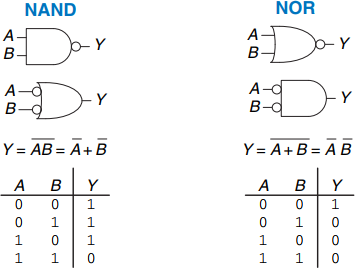
\includegraphics[width=0.5\textwidth]{de_morgan_gates.png}
    \caption{De Morgan equivalent gates and their truth tables}
    \label{figure:9}
\end{figure}

Figure~\ref{figure:10} was selected for showing the drastic hardware reduction using multilevel combinational logic. Normally, to construct an eight-input XOR gate, there would be 128 eight-input AND gates and one 128-input OR gate. Nevertheless, using the associative property of XOR, $A \oplus B \oplus C = (A \oplus B) \oplus C$, an eight-input XOR gate can also be produced by using a tree of seven two-input XOR gates. There is a huge difference in hardware monetary cost and hardware space cost between the two methods of implementation.

\begin{figure}[h]
    \centering
    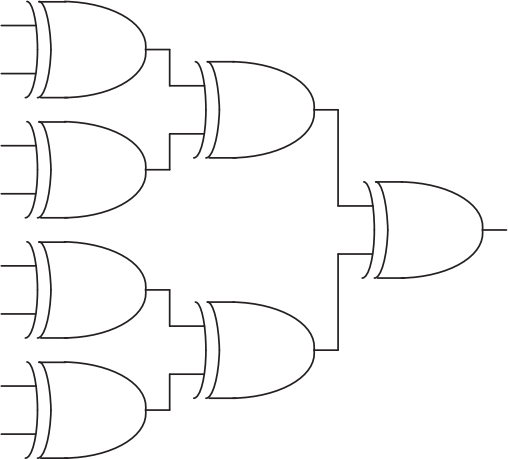
\includegraphics[width=0.25\textwidth]{eight_input_xor}
    \caption{An eight-input XOR constructed from seven two-input XOR}
    \label{figure:10}
\end{figure}

%%%%%%%%%%%%%%%%%%%%%%%%%%%%%%%%%%%%%%%%%%%%%%%%%%%%%%%%%%%%%%%%%%%%%%%%%%%%%%%%
% Example Problems
%%%%%%%%%%%%%%%%%%%%%%%%%%%%%%%%%%%%%%%%%%%%%%%%%%%%%%%%%%%%%%%%%%%%%%%%%%%%%%%%
\section{Example Problems}

See the attached PDF \textit{Luu\_Chapter2\_Example\_Problems.pdf}.

%%%%%%%%%%%%%%%%%%%%%%%%%%%%%%%%%%%%%%%%%%%%%%%%%%%%%%%%%%%%%%%%%%%%%%%%%%%%%%%%
% Glossary
%%%%%%%%%%%%%%%%%%%%%%%%%%%%%%%%%%%%%%%%%%%%%%%%%%%%%%%%%%%%%%%%%%%%%%%%%%%%%%%%
\section{Glossary}

All definitions were found from the Google search engine, typing "circuit dictionary" for the first item.

\begin{enumerate}
    \item Circuit

    noun:

    \begin{enumerate}
        \item a roughly circular line, route, or movement that starts and finishes at the same place.
        \item an established itinerary of events or venues used for a particular activity, typically involving public performance.
    \end{enumerate}

    verb:

    \begin{enumerate}
        \item move all the way around (a place or thing).
    \end{enumerate}

    \item Boolean

    adjective:

    \begin{enumerate}
        \item denoting a system of algebraic notation used to represent logical propositions, especially in computing and electronics.
    \end{enumerate}

    noun:

    \begin{enumerate}
        \item a binary variable, having two possible values called ``true" and ``false."
    \end{enumerate}

    \item{Combination}

    noun:

    \begin{enumerate}
        \item a joining or merging of different parts or qualities in which the component elements are individually distinct.
        \item a sequence of numbers or letters used to open a combination lock.
    \end{enumerate}

    \item{Axiom}

    noun:

    \begin{enumerate}
        \item a statement or proposition that is regarded as being established, accepted, or self-evidently true.
    \end{enumerate}

    \item{Theorem}

    noun:

    \begin{enumerate}
        \item a general proposition not self-evident but proved by a chain of reasoning; a truth established by means of accepted truths.
    \end{enumerate}
\end{enumerate}

%%%%%%%%%%%%%%%%%%%%%%%%%%%%%%%%%%%%%%%%%%%%%%%%%%%%%%%%%%%%%%%%%%%%%%%%%%%%%%%%
% Interview Question
%%%%%%%%%%%%%%%%%%%%%%%%%%%%%%%%%%%%%%%%%%%%%%%%%%%%%%%%%%%%%%%%%%%%%%%%%%%%%%%%
\section{Interview Question}

See the attached PDF \textit{Luu\_Chapter2\_Interview\_Question.pdf}.

%%%%%%%%%%%%%%%%%%%%%%%%%%%%%%%%%%%%%%%%%%%%%%%%%%%%%%%%%%%%%%%%%%%%%%%%%%%%%%%%
% Reflection
%%%%%%%%%%%%%%%%%%%%%%%%%%%%%%%%%%%%%%%%%%%%%%%%%%%%%%%%%%%%%%%%%%%%%%%%%%%%%%%%
\section{Reflection}

I believe it is important to understand this chapter's materials well because this chapter establishes the idea of circuits, logic, and schematics and connects mathematics and physics to circuit design. Since I'm a Computer Science student who has a hobby in building circuits and making small robots, I found Boolean algebra, combinational circuits, and logic simplification quite interesting. What impressed me the most in this chapter was the Karnaugh map. I will definitely use the map as a graphical and intuitive way to double-check the correctness when I simplify logic functions.

The Boolean algebra and Karnaugh maps sections of the chapter were fairly easy. Though, I'm still trying to make sense of the multiplexer and the tristate buffer and their applications in circuit design. I am looking forward to learn more about combinational circuits, hardware reduction, and combinational building blocks in lecture.

%%%%%%%%%%%%%%%%%%%%%%%%%%%%%%%%%%%%%%%%%%%%%%%%%%%%%%%%%%%%%%%%%%%%%%%%%%%%%%%%
% Questions for Lecture
%%%%%%%%%%%%%%%%%%%%%%%%%%%%%%%%%%%%%%%%%%%%%%%%%%%%%%%%%%%%%%%%%%%%%%%%%%%%%%%%
\section{Questions for Lecture}

\begin{enumerate}
    \item What are the applications of multiplexers? Can you show me a real-life example of a multiplexer?
    \item What determines which input will be taken into account in a tristate buffer?
    \item Electronic devices, such as smartphones, are getting smaller and faster but also more expensive. Do you favor speed or cost?
\end{enumerate}

%%%%%%%%%%%%%%%%%%%%%%%%%%%%%%%%%%%%%%%%%%%%%%%%%%%%%%%%%%%%%%%%%%%%%%%%%%%%%%%%
% Bibliography
%%%%%%%%%%%%%%%%%%%%%%%%%%%%%%%%%%%%%%%%%%%%%%%%%%%%%%%%%%%%%%%%%%%%%%%%%%%%%%%%
\bibliographystyle{ieeetr}
\bibliography{references}

\end{document}
